\documentclass[a4paper,english]{article}
\usepackage[margin=1in]{geometry}
\usepackage[utf8x]{inputenc}
\usepackage{afterpage}
\usepackage{xcolor}
\usepackage{pdfpages}
\usepackage{graphicx}
\usepackage{subfig}
\usepackage{caption}
\usepackage[english]{babel}

\usepackage[toc,page]{appendix}
\usepackage[square,numbers]{natbib}
\bibliographystyle{abbrvnat}

\usepackage{expl3}
\expandafter\def\csname ver@l3regex.sty\endcsname{}
\usepackage{coloremoji}

%\usepackage[outputdir=./tmp,newfloat]{minted} % need to call 
%<pdflatex -shell-escape>

%% by overleaf %%
\usepackage{listings}
%New colors defined below
\definecolor{codegreen}{rgb}{0,0.6,0}
\definecolor{codegray}{rgb}{0.5,0.5,0.5}
\definecolor{codepurple}{rgb}{0.58,0,0.82}
\definecolor{backcolour}{rgb}{0.95,0.95,0.92}
\definecolor{mylinkcolor}{rgb}{.2, .3, .9}
%Code listing style named "mystyle"
\lstdefinestyle{mystyle}{
	backgroundcolor=\color{backcolour},
	commentstyle=\color{codegreen},
	keywordstyle=\color{magenta},
	numberstyle=\tiny\color{codegray},
	stringstyle=\color{codepurple},
	basicstyle=\ttfamily\footnotesize,
	breakatwhitespace=false,         
	breaklines=true,             
	captionpos=b,                    
	keepspaces=true,                 
	numbers=left,                    
	numbersep=5pt,                  
	showspaces=false,                
	showstringspaces=flase,
	showtabs=false,              
	tabsize=2
}
%"mystyle" code listing set
\lstset{style=mystyle}


\usepackage{fancyhdr}
\pagestyle{fancy}
\fancyhf{} 	% it clears the header and footer of default "plain" page style
\lhead{\leftmark}
\rhead{\thepage}
\chead{\hyperlink{Contents}{Contents}}

\usepackage{hyperref, bookmark}

\hypersetup{
	pdftitle = {FEM for TPBVP},
	pdfsubject = {Finite Element Method},
	pdfauthor = {Mark Taylor},
	bookmarks = true,
	bookmarksnumbered = true,
	pdfpagelabels = true,
	pdfpagemode = UseOutlines,
	pdfstartview = FitH,
	linktocpage = true,
	colorlinks = true,
	linkcolor = mylinkcolor,
	urlcolor = magenta,
	plainpages = false
}

\linespread{1.1}

\begin{document}
	% cover page
	\thispagestyle{empty}
	\begin{figure}
		\centering
		
\includegraphics[width=0.81\paperwidth]{img/lion.png}
		\caption*{\href{https://github.com/How-u-doing}{how U doin'?}
			\\ $🐳^{🐳^{🐳}} = ∫_{🎃}^{🎅} 🐑 \ d🍀$ }
		\label{cover:lion}
	\end{figure}
	\pagecolor{pink}
	\afterpage{\nopagecolor}
	\clearpage
	\newpage
	
	\title{FEM for TPBVP \thanks{This article was typeset by Mark Taylor using 
	the \protect\LaTeX{} document processing system.}}
	
	\author{10170437 Mark Taylor}
	
	\date{December 18, 2020}
	
	\maketitle
	
	\hypertarget{Contents}{}  % Make an anchor to the toc
%	\phantomsection  % optional
	\pdfbookmark[1]{\contentsname}{Contents}    % at current level (== 1)
%	\belowpdfbookmark{\contentsname}{Contents}  % equivalent to above one
	\tableofcontents
	
	\clearpage
	
	\section{Problems}
		
	\begin{figure}[!hb]
		\centering
		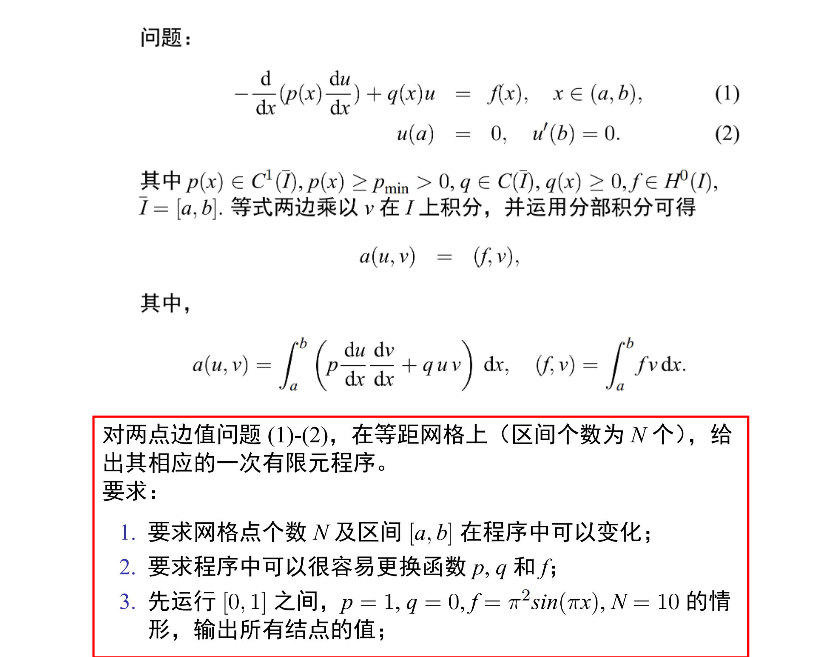
\includegraphics[width=0.7\linewidth]{img/problem}
		\caption*{}
		\label{fig:problem}
	\end{figure}

	
	\section{Theory }
	See 
	\href{https://github.com/How-u-doing/Numerical_Analysis/blob/master/Chapter10_BVPforODEs/reference.mlx}{reference.mlx}
	\cite{NA9e}  and 
	\href{https://github.com/How-u-doing/Numerical_Analysis/blob/master/Chapter10_BVPforODEs/error_analysis.mlx}{error\_analysis.mlx}
	\cite{chap5}	in the \emph{src} folder.
	Our text \cite{LiRonghua} also has a very detailed analysis on
	FEM error estimates.
	
	
	\section{Solutions}	
	🔑 🔑 🔑 \\[5pt]	
	See graphs of those two test problems as follows. View code 
	\hyperref[Code]{here💻}.
	
	\clearpage

	\begin{figure}[!hb]
		\makebox[\textwidth][c]{			
			\subfloat[Problem 1 by PLRR]
			{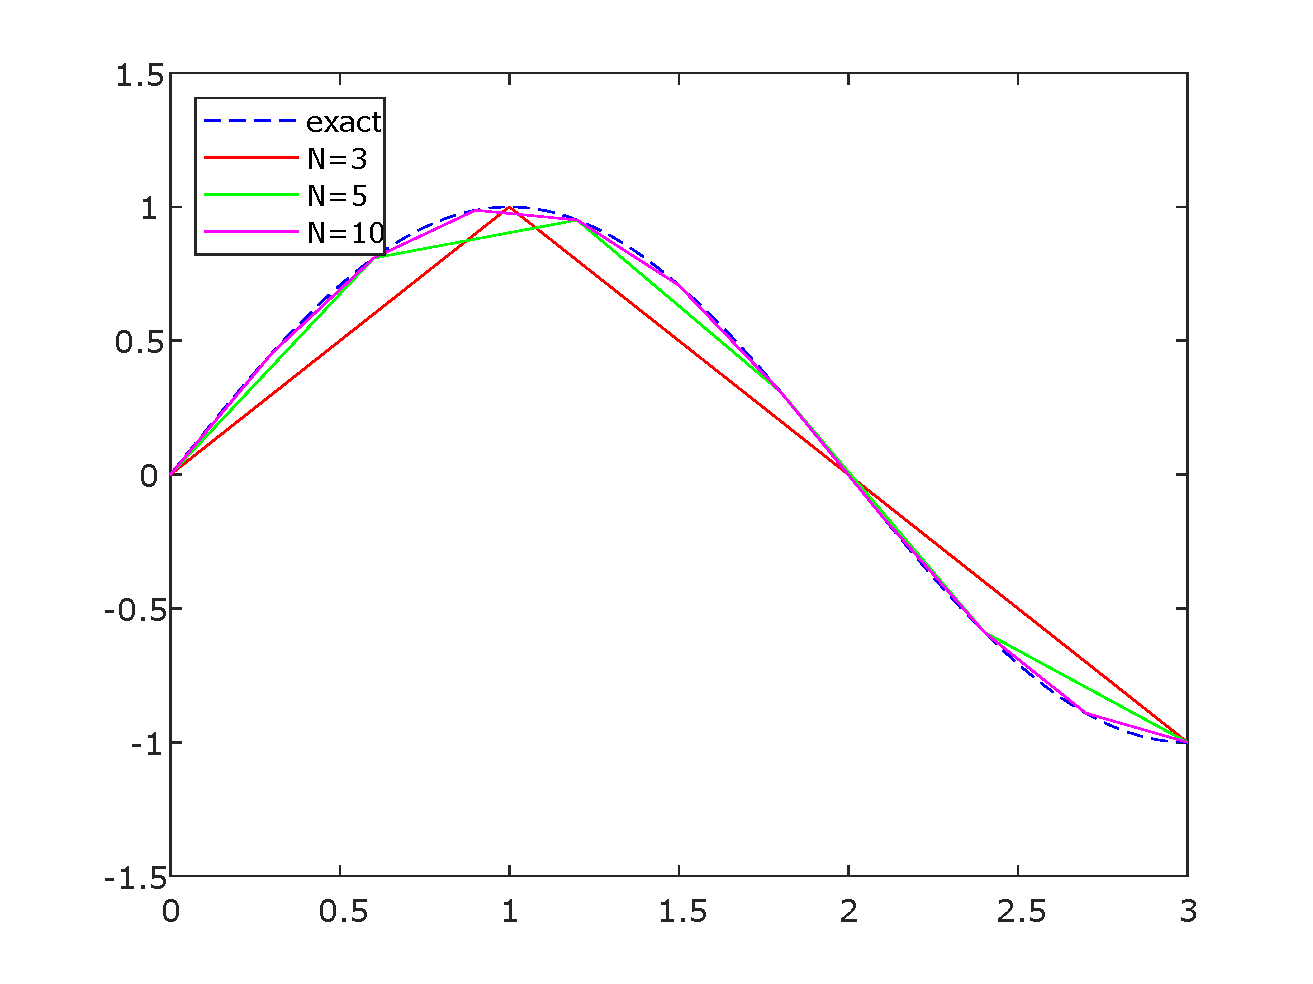
\includegraphics[width=0.47\paperwidth]{svg/problem_1_[0,3]}}
			\subfloat[Problem 1 by PQRR]
			{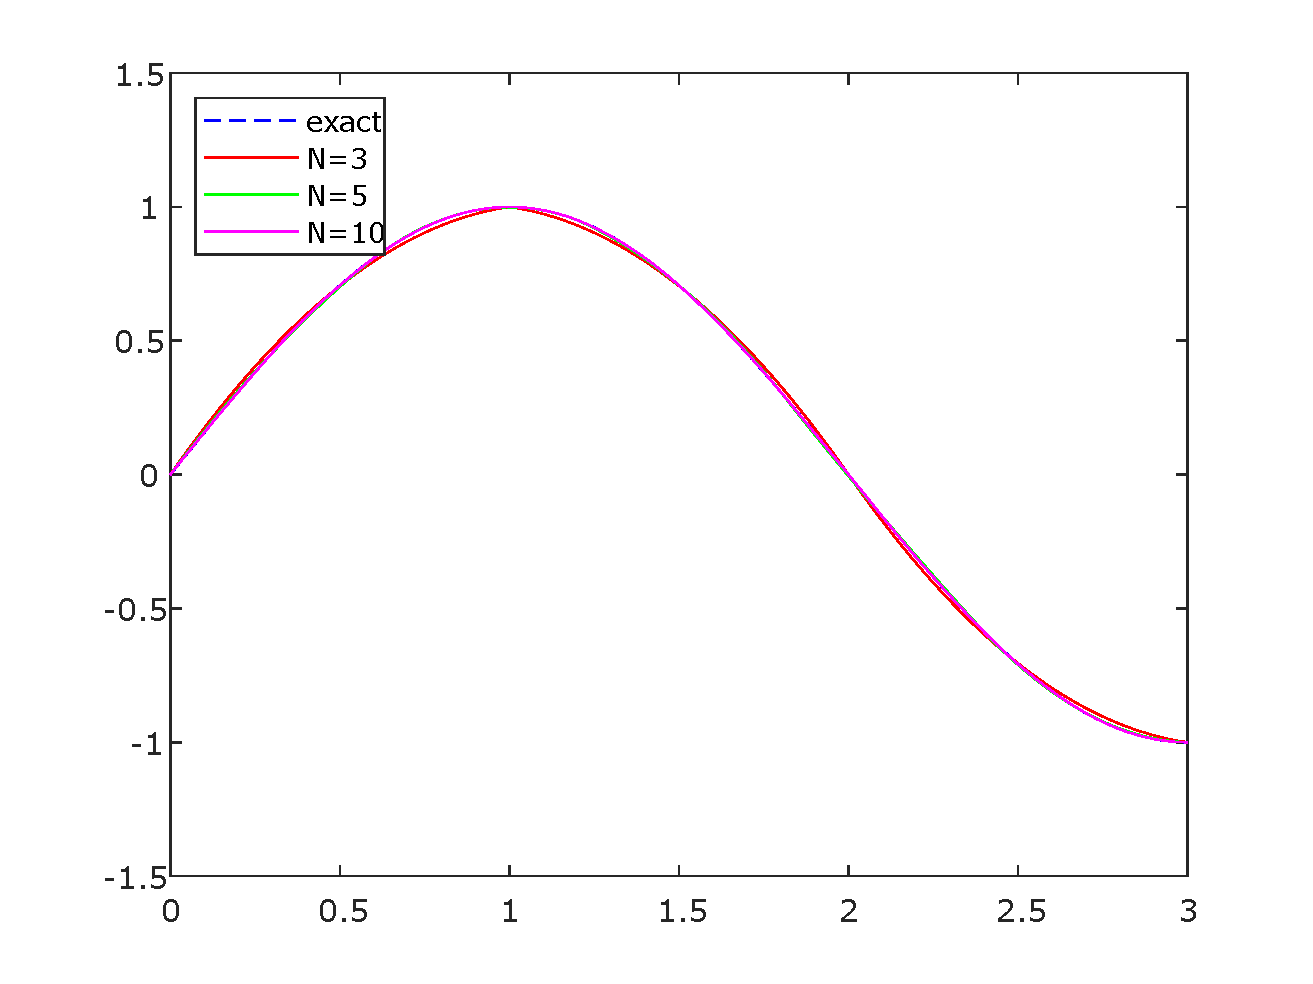
\includegraphics[width=0.47\paperwidth]{svg/problem_1_[0,3]_quad}}
		}\\
		\makebox[\textwidth][c]{
			\subfloat[Problem 2 by PLRR]
			{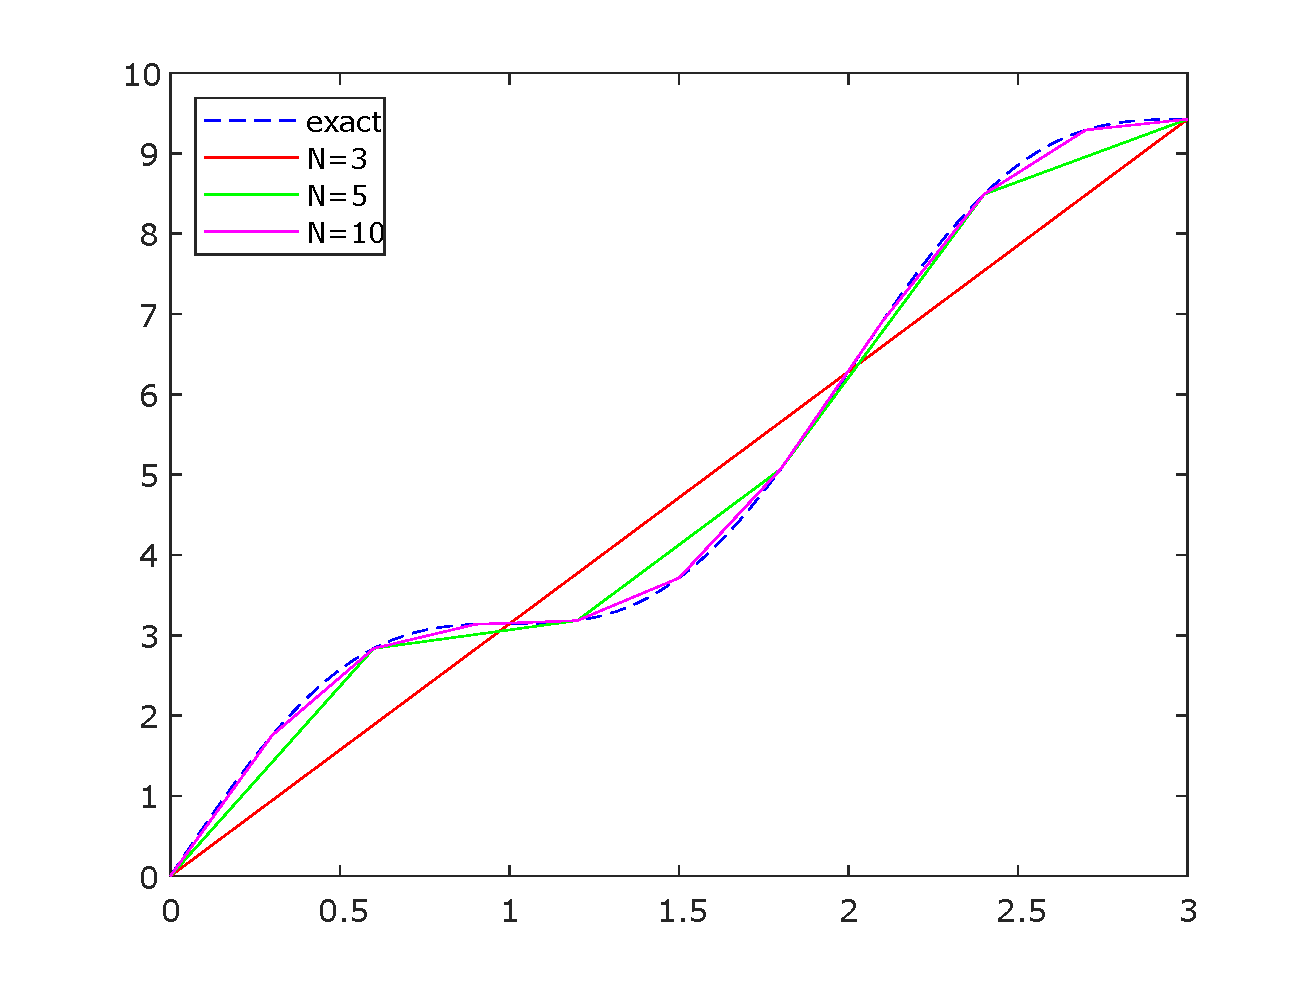
\includegraphics[width=0.47\paperwidth]{svg/problem_2_[0,3]}}
			\subfloat[Problem 2 by PQRR]
			{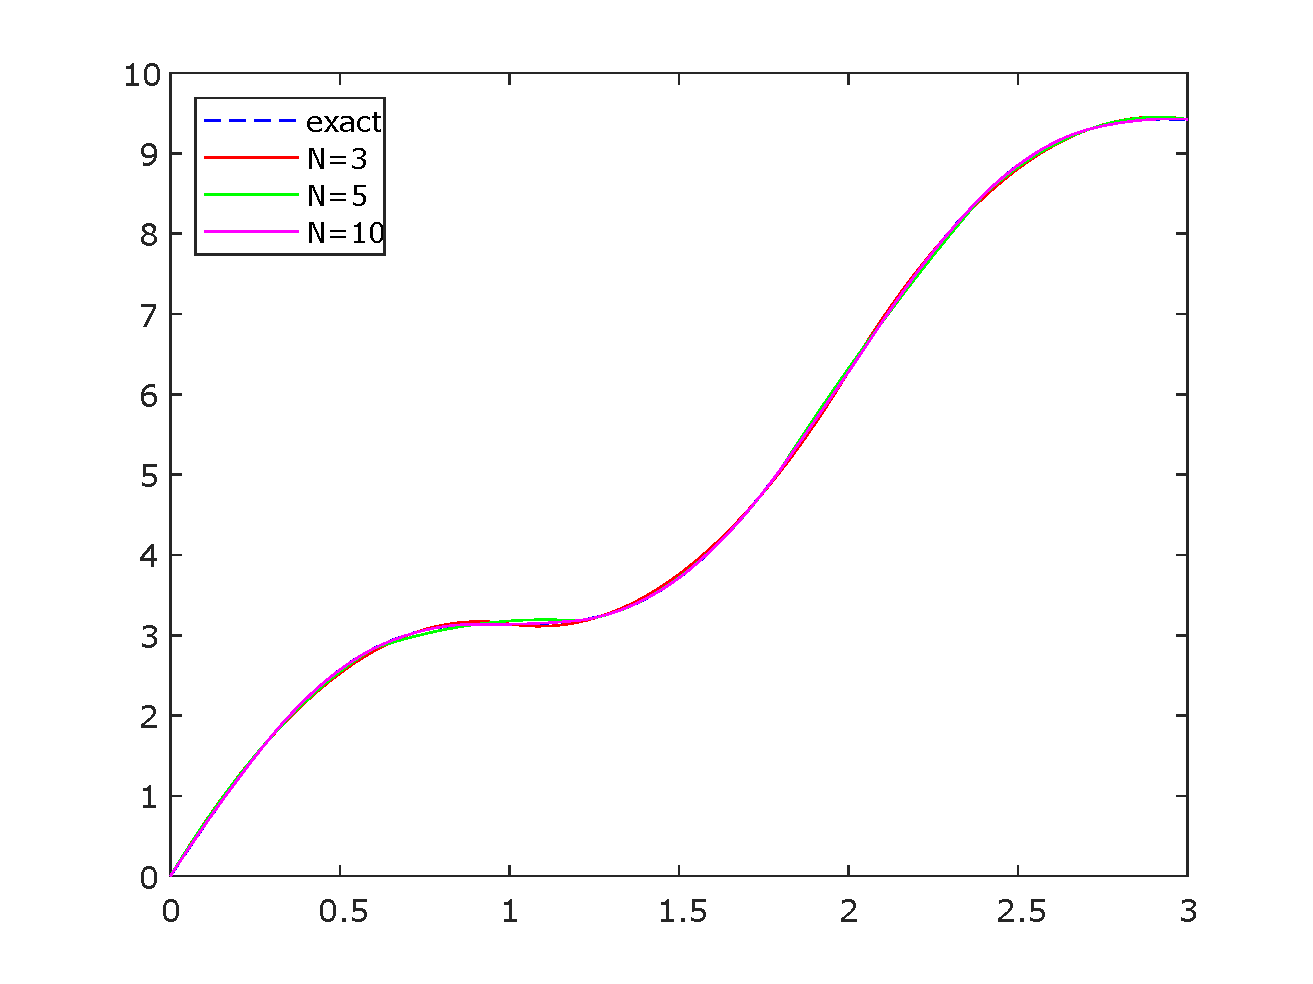
\includegraphics[width=0.47\paperwidth]{svg/problem_2_[0,3]_quad}}
		}	
		\caption{Fittings via \hyperref[PLRR]{PLRR} \& \hyperref[PQRR]{PQRR}}
	\end{figure}

	\begin{figure}[!hb]
		\makebox[\textwidth][c]{
			{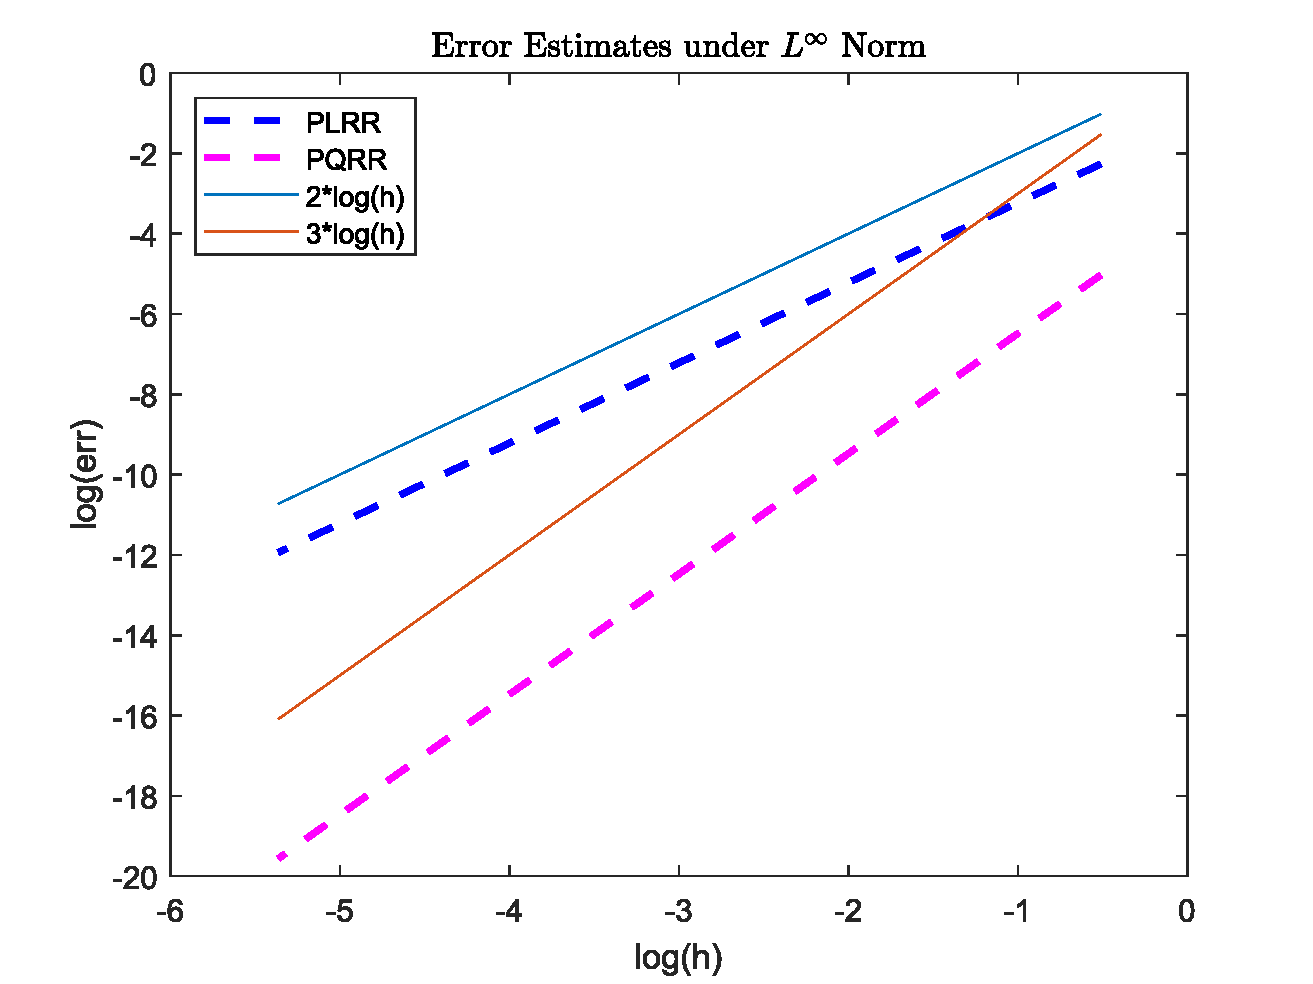
\includegraphics[width=0.31\paperwidth]{svg/L_inf_norm}}
			{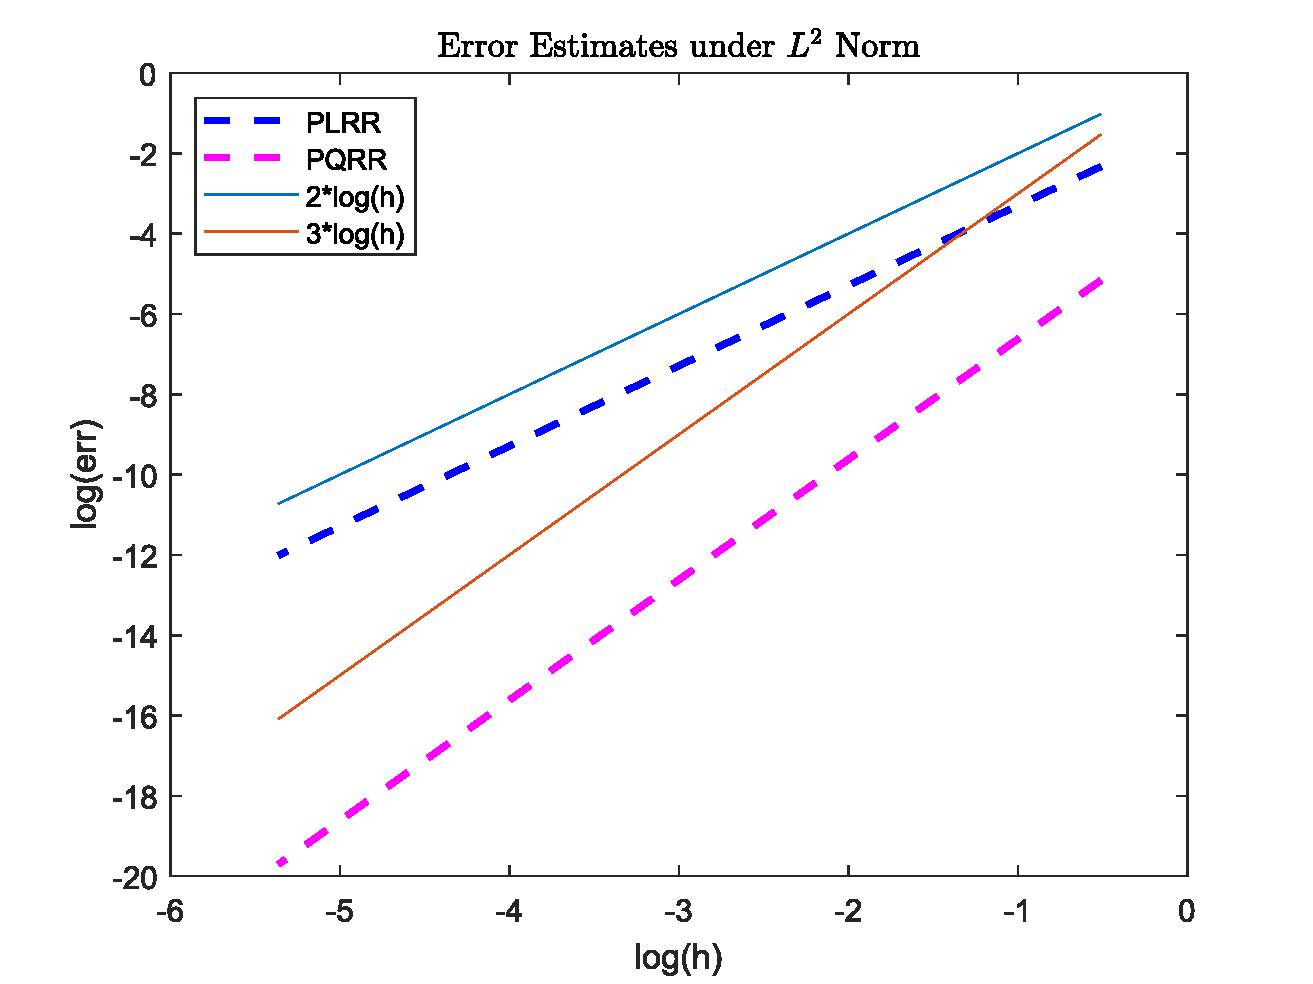
\includegraphics[width=0.31\paperwidth]{svg/L_2_norm}}
			{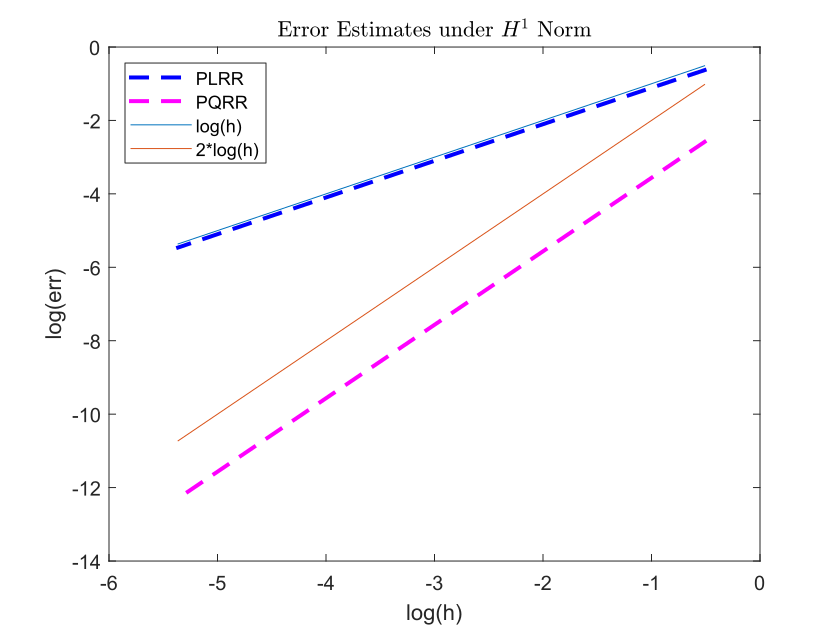
\includegraphics[width=0.31\paperwidth]{svg/H_1_norm}}
		}
		\caption{1-d FEM \hyperref[error_estimates]{error estimates} under 
		different norms}
	\end{figure}

	\clearpage
	

	\section{Code}\label{Code}
	
	\subsection{Scripts (Main Functions)}
	% use minted package
	%\begin{listing}[ht]
	%	\inputminted{octave}{src/PLRR_test.m}
	%	\caption{PLRR_test for solving two-point BVP}
	%	\label{PLRR_test}
	%\end{listing}
	
	\lstinputlisting[language=Octave, 
	caption={PLRR\_test for solving two-point BVP},
	label=PLRR_test
	]{src/PLRR_test.m}
	
	\lstinputlisting[language=Octave, 
	caption={PQRR\_test for solving two-point BVP},
	label=PQRR_test
	]{src/PQRR_test.m}
	
	
	\subsection{Error Estimates}
	\lstinputlisting[language=Octave, 
	caption={Error Estimates for FEM},
	label=error_estimates
	]{src/error_estimates.m}
	
	
	\subsection{PLRR and PQRR}
	These are the exact methods we used for solving this 
	two-point boundary value problem.
	
	\lstinputlisting[language=Octave, 
	caption={Piecewise Linear Rayleigh-Ritz method},
	label=PLRR
	]{src/PLRR.m}
	
	\lstinputlisting[language=Octave, 
	caption={Piecewise Qudratic element Rayleigh-Ritz method
		global stiffness matrix version},
	label=PQRR
	]{src/PQRR.m}
	
	\lstinputlisting[language=Octave, 
	caption={Piecewise Qudratic element Rayleigh-Ritz method
				element stiffness matrix version},
	label=PQRR_es
	]{src/PQRR_es.m}	
	
	
	\subsection{PLRR\_intpol and PQRR\_intpol}
	Interpolations for PLRR and PQRR.
	
	\lstinputlisting[language=Octave, 
	caption={Interpolation for PLRR} ,
	label=PLRR_intpol
	]{src/PLRR_intpol.m}
	
	\lstinputlisting[language=Octave, 
	caption={Interpolation for PQRR} ,
	label=PQRR_intpol
	]{src/PQRR_intpol.m}
	
	
	\subsection{Gaussquad}
	This is a usr-defined function that servers the purpose of 
	numerical integration, which can be simply identically substituted by
	MATLAB build-in function \emph{integral}.
	
	\lstinputlisting[language=Octave, 
	caption={Gaussian quadrature} ,
	label=Gaussquad
	]{src/Gaussquad.m}
	
	\subsection{GauEli}
	A routine for solving linear equations of the form $Ax=b$.
	
	\lstinputlisting[language=Octave, 
	caption={Gaussian Elimination} ,
	label=GauEli
	]{src/GauEli.m}
	
	
	\medskip
	
	%% References
	\bibliography{bibliography.bib}
	\addcontentsline{toc}{section}{References}


	%% Appendices
	\appendix
	\section*{Appendices}
	\addcontentsline{toc}{section}{Appendices}
	
	\begin{figure}[!hb]
		\centering
		\includegraphics[width=1\linewidth]{\string"img/The 
		Beatles\string".jpg}
		\caption*{Hello from the Beatles.😃}
		\label{fig:the-beatles}
	\end{figure}
	
\end{document}
